%\documentclass[a4paper,10pt,twoside]{article}
\documentclass[10pt,a4paper,twoside]{llncs}
\usepackage[left=3cm,right=3cm,top=2.5cm,bottom=2.5cm]{geometry}
\setcounter{secnumdepth}{5}%to set numbering over subsubsections
%\usepackage[utf8x]{inputenc}
\usepackage[T1]{fontenc}
\usepackage[latin1]{inputenc}
\usepackage{amsmath,amsfonts,amssymb}%\usepackage{amsmath,amsfonts,amsthm,amssymb}
\usepackage{graphicx}
\usepackage{pstricks}    %for embedding pspicture.
\usepackage{epsfig}
\usepackage{algorithmic,algorithm}
\usepackage[colorlinks=true,linkcolor=blue,urlcolor=blue,citecolor=blue]{hyperref}
%\usepackage{tikz}
%\usetikzlibrary{matrix}

\pagestyle{headings}%page numbers



\usepackage{enumitem}
\setlistdepth{5}
\setlist[itemize,1]{label=-}
\setlist[itemize,2]{label=-}
\setlist[itemize,3]{label=-}
\setlist[itemize,4]{label=-}
\setlist[itemize,5]{label=-}
\renewlist{itemize}{itemize}{5}

% \newcounter{subsubparagraph}[subparagraph]
% \renewcommand\thesubsubparagraph{\thesubparagraph.\@arabic\c@subsubparagraph}
% \newcommand\subsubparagraph{\@startsection{subsubparagraph}{6}{\parindent}%
%                                        {3.25ex \@plus1ex \@minus .2ex}%
%                                        {-1em}%
%                               {\normalfont\normalsize\bfseries}}
% \newcommand*\l@subsubparagraph{\@dottedtocline{6}{10em}{5em}}

%%%%%%%%%%%%%%%%%%%%%%%%%%% VERSIONES %%%%%%%%%%%%%%%%%%%%%%%%%%%%%%%%%%%
%\usepackage{gitinfo}
%\newcommand{\version}{github.Papers: \gitCommitterDate\;(revision \gitAbbrevHash) } %!!fixme!!
\newcommand{\version}{github.Papers: 2013-09-30\;(revision \_\_\_\_\_\_\_\_) } %git log -n 1 --pretty=format:"%H"
\newcommand{\todo}[1]{\texttt{\color{red}TODO:} ``\emph{#1}''}
\newcommand{\fixme}[1]{\texttt{\color{red}FIXME:} ``\emph{#1}''}
%%%%%%%%%%%%%%%%%%%%%%%%%%%%%%%%%%%%%%%%%%%%%%%%%%%%%%%%%%%%%%%%%%%%%%%%%
\newcommand{\tango}{\textsc{Tango}}
\newcommand{\sardana}{\textsc{Sardana}}
\newcommand{\taurus}{\textsc{Taurus}}
\newcommand{\atk}{\textsc{Atk}}
\newcommand{\zmq}{\textsc{$\varnothing$mq}}
\newcommand{\corba}{\textsc{Corba}}
\newcommand{\mambo}{\textsc{Mambo}}
\newcommand{\lima}{\textsc{Lima}}

%opening
\title{Securing \tango\, Control System: A brain storming}
\author{Sergi Blanch-Torn\'e\inst{1}, Josep Maria Miret Biosca\inst{2}, Ramiro Moreno Chiral\inst{2}, Francesc Seb\'e Feixa\inst{2}}
 \institute{
 Escola Polit\`ecnica Superior, Universitat de Lleida. Spain.\\
 \email{\tt sblanch@alumnes.udl.es}
 \and 
 Departament de Matem\`atica. Universitat de Lleida. Spain.\\
 \email{\tt \{miret,ramiro,fsebe\}@matematica.udl.es}
 }
%% TODO; Fernando Cores can help a lot in this project


%%% Definiciones matem\'aticas especiales

\newcommand{\Z}{\ensuremath{\mathbb{Z}}}%                       Enteros
\newcommand{\Q}{\ensuremath{\mathbb{Q}}}%                       Racionales
\newcommand{\A}{\ensuremath{\mathcal{A}_{2}}}%                   Plano Af\'{\i}n
\newcommand{\Proy}{\ensuremath{\mathcal{P}_{2}}}%                Plano Proyectivo
\newcommand{\Jacob}{\ensuremath{\mathcal{J}_{2}}}%               Plano Jacobiano
\newcommand{\K}{\ensuremath{\mathbb{K}}}%                       Cuerpo en general
\newcommand{\F}{\ensuremath{\mathbb{F}}}%                       Cuerpo finito en general
\newcommand{\Fp}{\ensuremath{\mathbb{F}_p}}%                    Cuerpo finito de orden p (primo)
\newcommand{\EFp}{\ensuremath{E(\mathbb{F}_p)}}%                Curva el\'\{i}ptica sobre un cuerpo finito de orden p (primo)
\newcommand{\EFq}{\ensuremath{E(\mathbb{F}_q)}}%                Curva el\'\{i}ptica sobre un cuerpo finito
\newcommand{\Fm}{\ensuremath{\mathbb{F}_{2^m}}}%                Cuerpo finito de caractar\'{\i}stica 2, grado m
\newcommand{\EFm}{\ensuremath{E(\mathbb{F}_p)}}%                Curva el\'\{i}ptica sobre un cuerpo finito de caractar\'{\i}stica 2, grado m
\newcommand{\Fq}{\ensuremath{\mathbb{F}_q}}%                    Idem id. q (q=p^m, p primo y m entero pos.)
\newcommand{\Zn}[1]{\ensuremath{\mathbb{Z}/#1\mathbb{Z}}}%      Anillo de los enteros mod n
\newcommand{\PaI}{\ensuremath{\mathcal{O}}}%                    Punto en el Infinito
\newcommand{\PaIe}{\ensuremath{\mathcal{O}_{E}}}%               Punto en el Infinito de la curva

%%% Algorithm customization:
%\floatname{algorithm}{Procedure}%Rename the text ``Algorithm''
\renewcommand{\algorithmicrequire}{\textbf{Input:}}
\renewcommand{\algorithmicensure}{\textbf{Output:}}
%%% end algorithm

\begin{document}

\maketitle
\begin{center}
 \today\\
 \version
\end{center}


\begin{abstract}\footnote{Partially supported by grants MTM2010-21580-C02-01 (Spanish Ministerio de Ciencia e Innovaci\'on), 2009SGR-442 (Generalitat de Catalunya).}

Current use of \tango\, is mostly in Synchrotron and recently extending it into a neutron source, but industry has expressed a desire to participate in the community. This industry desire has been made with concern on security. Not a concern in IT environmental, that is institution/user choose, it was about the use of cryptology to mathematically protect the system.

The goal of ensure \tango\, must produce an outcome as similar as the \emph{TLS} is for the web navigation. Must be possible to co-live with non secured access, but with a tendency to a complete transparent ensuring. Perhaps the migration process would be not as fast as we could want, specially due to the introduction of the certificates infrastructure, but as the \tango\, installations are contained in the institutions, and upgrade in this way would be like any other upgrade.

Also as web navigation did, \tango\, is used with instances running over different architectures and operating systems, from small embedded devices, up to very big computers. Then the objective in this ensuring process is that must work just as for the larger than for the tiny.

It is very important goal to have the \tango\, implementation as Free Software, as this paper cryptography outcomes must be to have public access with auditable algorithms and sources.
   
{\bf Keywords:} Cryptography\footnote{This big keyword includes proposals over \emph{Public key}, \emph{Elliptic Curves}, \emph{Symmetric algorithms}, \emph{stream cyphers}, \emph{secret sharing} and also \emph{Homomorphic encryption} for databases.}, Distributed Control Systems, Cryptography engineering.

\end{abstract}

%%%%%%%%%%%%%%%%%%%%%%%%%%%%%%%%%%%%%%%%%%%%%%%s
\section{Introduction \label{sec:introduction}}


\begin{itemize}
    \item Definition of an \emph{Industrial Control System} (ICS). And definition of what is included under this definition, namely: \emph{Programmable Logic Controllers} (PLC), \emph{Supervisory Control And Data Acquisition} (SCADA) and \emph{Distributed Control System} (DCS).
    \item Define \emph{Distributed system} and \emph{Middleware} \cite{TanenbaumDistr}.
    \item \tango\, definition as a DCS. \tango\, as a PLC wrapper. Describe the \tango\, Consortium and its (9) members. Remark its \emph{Free software} licensing and repositories in \emph{sourceforge}. \tango-core (the middlelayer) is LGPLv3 and the agents in the distributed system in the \tango-DeviceServer repository are GPLv3.
    \begin{itemize}
        \item Define DeviceServer
        \item Define DeviceClass
        \item Define Device
    \end{itemize}
    \item auxiliary pieces that with \tango\, extends their uses: \atk, \sardana\, and \taurus\, to build SCADAs. \mambo\, as data archiver.
    \item \tango\, as a middleware: \corba\, (\emph{omniORB} 4.1 \cite{omniORB41}) for the synchronous and asynchronous, and \zmq\, (3.2 \cite{zmq32}) for the event based communication.
    \item View \tango\, middleware as the basic brick to have \emph{transportation} layer (from the OSI schema) in the DCS. The \emph{session} layer is almost uncovered with shiny skills in \atk, \sardana\, and \taurus.
    \item \fixme{Is the security within \atk, \sardana, \taurus\, and \mambo, included in this paper?}
    \item \todo{Other complementary tools like \lima?}
    \item Last \tango-meeting (the 27th) (aerospace) industry (Onera), beyond the scientific research currently using \tango, request to improve the security skills of \tango.
    \item There is a broad spectrum of potential stakeholders with a huge request on security, in terms of cryptography, like energy generation and delivery, home automation, car manufacturers, and many more.
    \begin{itemize}
        \item \tango\, needs the 's' as happened to https, stmps, imaps, telnet (ssh),...
    \end{itemize}
    \item The competitors of \tango, neither have much security skills.
    \item
    \item
\end{itemize}

\begin{figure}[h]
    \centering{
        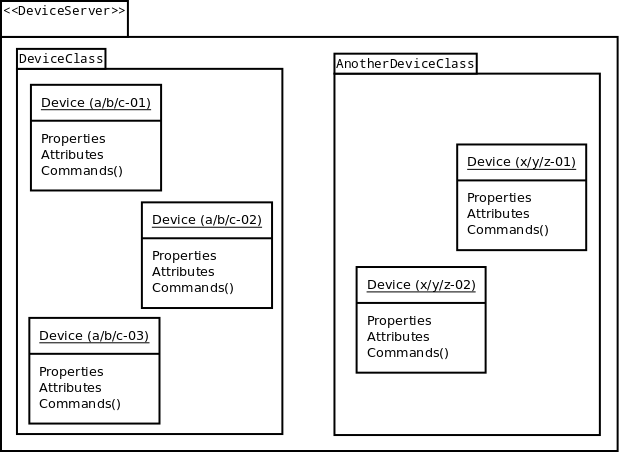
\includegraphics[width=0.7\textwidth]{imgs/tango/tango_DeviceServer_DeviceClass_Device.png}
        \caption{Schematic view about the definition of the term DeviceServer, DeviceClass and Device, and Data information. \todo{This image must be improved}\label{fig:definitions}}
    }
\end{figure}

\begin{figure}[h]
    \centering{
        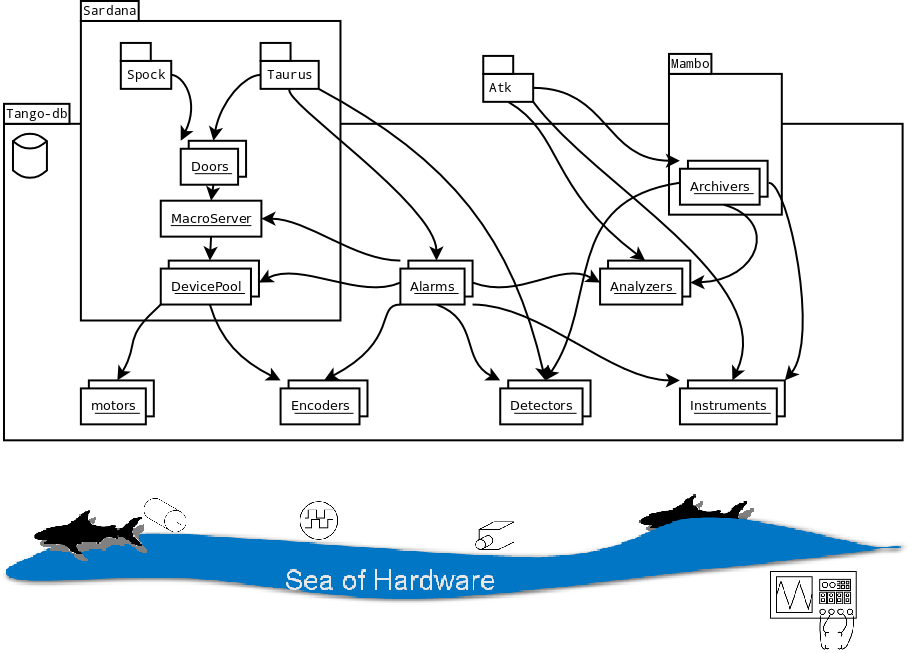
\includegraphics[width=0.75\textwidth]{imgs/tango/tango_layout.png}
        \caption{Tango schematic layout \todo{This image must be improved significantly}} \label{fig:tangoLayout}
    }
\end{figure}


%%%%%%%%%%%
\subsection{Defining distributed system security \label{sec:distributedSecuritySystems}}

\begin{itemize}
    \item What is the meaning of a secure system? What is security in a distributed system?
    \item The basics on \emph{information security}
    \begin{itemize}
        \item Confidentiality: Information must be disclosed only to the authorized.
        \item integrity: Only authorized can set in the system.
        \item Availability: Information must be accessible for those who are authorized.
        \item Authenticity: Information must only be emitted by the authorized.
        \item Non-repudiation: Forbid validity changes on the information emitters.
    \end{itemize}
    \item Add another brick
    \begin{itemize}
        \item Auditory: trace who access where (extremely useful for a security breach analysis).
    \end{itemize}
    \item
    \item
\end{itemize}


%%%%%%%%%%%
\subsection{Structure of the paper \label{sec:structurePaper}}

\begin{itemize}
    \item The structure of this paper starts with the definitions in the introduction (section \ref{sec:introduction})
    \item This is followed by a section to identify scenarios (section \ref{sec:scenarios}) that has a subsection with practical examples of the scenarios (\ref{sec:practExamples}) and the definition of a security thread (section \ref{sec:securityThreads}) over the identified scenarios.
    \item Next is to do a Brainstorming of the possible attacks (section \ref{sec:attacks}) starting from the fundamental environment security (section \ref{sec:environment}) followed by the passive and active attacks (sections \ref{sec:passiveAttacks} and \ref{sec:activeAttacks}), non forgetting the big thread that means implementation issues known as side channel attacks (section \ref{sec:sideChannelAttacks}). All attack study must contain countermeasures that are in section \ref{sec:countermeasures} with special emphasis on intrusion detection in section \ref{sec:intrusionDetection}.
    \item Central part of the paper is the section \ref{sec:CryptoEng} named ``Cryptography Engineering''. 
    \begin{itemize}
        \item First part with the application layering view from \cite{TanenbaumDistr} in section \ref{sec:layering} (presentation layer \ref{sec:presentationLayer}, domain layer \ref{sec:domainLayer} and data layer \ref{sec:dataLayer})
        \item Followed by the proposed solutions in section \ref{sec:propSolutions} that are split in:
        \begin{itemize}
            \item Authentication \ref{sec:authentication}
            \begin{itemize}
                \item Zero-knowledge proofs \ref{sec:zeroknown}
            \end{itemize}
            \item Encryption \ref{sec:encryption}
            \begin{itemize}
                \item Public key (Elliptic curves) \ref{sec:ecpk}
                \begin{itemize}
                    \item Secret sharing \ref{sec:secretSharing}
                \end{itemize}
                \item Symmetric ciphers \ref{sec:symmentrics}
                \item Stream ciphers \ref{sec:streamming}
                \begin{itemize}
                    \item Secret splitting \ref{sec:secretSplitting}
                \end{itemize}
            \end{itemize}
            \item Ordered cryptography \ref{sec:orderedCrypto}
            \begin{itemize}
                \item 
            \end{itemize}
        \end{itemize}
    \end{itemize}
    \item Conclusions section (\ref{sec:conclusions}) with a further work subsection (\ref{sec:further})
    \item
    \item
\end{itemize}


%%%%%%%%%%%%%%%%%%%%%%%%%%%%%%%%%%%%%%%%%%%%%%%%%%%%%
\section{Identifying scenarios \label{sec:scenarios}}

\begin{itemize}
    \item Securing communications between RFID cards and an authorized reader \cite{Santi11} would be not too different than communication between two agents in a distributed system or between and agent and the element in the presentation layer.
    \item From the view from \cite{TanenbaumDistr} over the distributed system transparencies:
    \begin{itemize}
        \item What is implemented in \tango\, and what is not? And why?
        \item Is any of the ``nots'' necessary to ensure a quality service.
    \end{itemize}
    \begin{table}
        \centering{
        \begin{tabular}{|l|l|}
            \hline
            Access & Hide differences in data representation and how a resource is accessed \\ \hline
            Location & Hide where a resource is located \\ \hline
            Migration & Hide that a resource may move to another location \\ \hline
            Relocation & Hide that a resource may be moved to another location while in use \\ \hline
            Replication & Hide that a resource is replicated \\ \hline
            Concurrency & Hide that a resource may be shared by several competitive users \\ \hline
            Failure & Hide a faulure and recovery of a resource \\ \hline
            Persistence & Hide whether a (software) resource is in memory or on disk \\ \hline
        \end{tabular}
        \caption{Distributed systems transparencies from \cite{TanenbaumDistr} \label{tab:transparencies}}}
    \end{table}
    \item In terms of security threads, what it's call ``\emph{thread modeling}'' which is more representative from \cite{SecEngRossAnderson} for the current use case? Gather information also from \cite{cryptoEngineering}
    \begin{itemize}
        \item Three may types: \emph{Hospital}, \emph{Bank}, \emph{Military Base} (from where the security threads usually comes from).
        \item Practical paranoia \cite{PractCryptoSchneier}:
        \item Identify threads
        \item Capability attack scenario
    \end{itemize}
    \item Cryptosystem configuration, security levels and information classification. Section \ref{sec:secLevel}. Can be saw as the nowadays number of rotors from the times of the electro-mechanical machines of last century.
    \item Setup \& Public-Key distribution protocols \cite{SecEngRossAnderson} sec.3.7.2
    \item Cryptosystem setup reset.
    \item Secret Shared schemas for (k,n)-to decrypt or (k,n)-signants. Section \ref{sec:secretSharing}.
    \item multicast and events (\zmq) can be scenarios of secret splitting. Section \ref{sec:secretSplitting}.
    \item 
    \item 
\end{itemize}


%%%%%%%%%%%
\subsection{Practical examples \label{sec:practExamples}}

\begin{itemize}
    \item The example of a laboratory use: Optics Lab \emph{Nanometer Optical Measuring-Long Term Profile} (NOM-LTP) for mirrors surface characterization in the angstr\"oms (1\AA{} = $1\times10^{-10}m$) range.
    \begin{itemize}
        \item 3 Hosts
        \item 12 DServers
        \item 19 DClasses
        \item 28 Devices
    \end{itemize}
    \item The example of a beamline use.
    \begin{itemize}
        \item 7 Hosts
        \item 34 DServers
        \item 82 DClasses
        \item 615 Devices
    \end{itemize}
    \item The example of an accelerator use with all the subsystems working together.
    \begin{itemize}
        \item 139 Hosts
        \item 1426 DServers
        \item 1551 DClasses
        \item 4259 Devices
    \end{itemize}
    \item Factories production lines
    \item Critical factories
    \item Traffic lights and tools
    \item Energy station
\end{itemize}

%%%%%%%%%%%
\subsection{Defining security threads \label{sec:securityThreads}}

\begin{itemize}
    \item Security threads, policies and mechanisms. Section \ref{sec:scenarios}. Go further that the Locking/Access control
    \item Why to secure it? Trust in a peripheral firewalls is not enough. Often communications between tango installations (different tango-db) requires firewall rules to allow it, but this doesn't allow to filter by agent or by who is allowed to access the information.
    \begin{itemize}
        \item In practice, what is filtered is an specific computer traffic, but this breaks many of the distributed system transparencies (section \ref{sec:scenarios}).
        \item The example of the Beamlines (read) access to (a few but crucial) accelerator information is a great example of what means a security thread.
        \item The industrial example of ``do it fast'' or ``finish it now'' more often than thought hides an insecure system or even worst a ``bugged'' system. 
    \end{itemize}
\end{itemize}


%%%%
\subsubsection{Security levels \label{sec:secLevel}}

\begin{itemize}
    \item Security levels: Open or unclassified, confidential, Secret, Top Secret. But an institution would like to define more than 4.
    \item Remember the \todo{German standard} on this levelling, the European commission ``\emph{fiche 17}'' \cite{fiche17EU}(``Exchange of EU classified information''), FIPS 140-2 \cite{NIST140-2}, Secure Sharing Suite S.3 \todo{document not yet found \cite{}}.
    \item Same security level would require an isolated environments. That is even if two subsystems have the same level, would be necessary to isolate threads between them.
    \item
    \item
\end{itemize}


%%%%%%%%%%%%%%%%%%%%%%%%%%%%%%%%%%%%%%%%%%%%%%%%%%%
\section{Brainstorming attacks \label{sec:attacks}}

\begin{itemize}
    \item This has relation with the scenarios identified in section \ref{sec:scenarios}. Specially what concerns the security thread types \cite{SecEngRossAnderson}.
    \item How mush work it takes to break the system? What's the value of the protected system?
    \item 
    \item
\end{itemize}


%%%%%%%%%%%
\subsection{Environmental IT Security \label{sec:environment}}

\begin{itemize}
    \item The weakest brick: secure the transmission but store in a plain file system
    \item Human behaviour and psychology.
    \item ISO/IEC 27000-series
    \item 
    \item
\end{itemize}


%%%%%%%%%%%
\subsection{Passive attacks \label{sec:passiveAttacks}}

\begin{itemize}
    \item Eavesdropping
    \item 
    \item 
\end{itemize}


%%%%%%%%%%%
\subsection{Active attacks \label{sec:activeAttacks}}

\begin{itemize}
    \item Men-in-the-middle (active attacks) between agents
    \item Spoofing: mask and falsify data
    \item Noise-Interruption-Poisoning: Break the public face, web site or gui. Kill a vital agent.
    \item Modification/Fabrication: Supplant agents.
    \item 
    \item 
\end{itemize}


%%%%%%%%%%%
\subsection{Side channel attacks \label{sec:sideChannelAttacks}}

\begin{itemize}
    \item
    \item 
\end{itemize}


%%%%%%%%%%
\subsection{Attacks countermeasures \label{sec:countermeasures}}

\begin{itemize}
    \item
    \item 
\end{itemize}


%%%%
\subsubsection{Intrusion Detection \label{sec:intrusionDetection}}

\begin{itemize}
    \item Detection and recovery
    \item 
    \item 
\end{itemize}


%%%%%%%%%%%%%%%%%%%%%%%%%%%%%%%%%%%%%%%%%%%%%%%%%%%%%%%%
\section{Cryptography Engineering \label{sec:CryptoEng}}

\begin{itemize}
    \item
    \item 
\end{itemize}


%%%%%%%%%%%
\subsection{Distributed system layering approach \label{sec:layering}}

\begin{itemize}
    \item
    \item 
\end{itemize}


%%%%
\subsubsection{Ensuring presentation layer \label{sec:presentationLayer}}

\begin{itemize}
    \item Agent authentication in a distributed system.
    \begin{itemize}
     \item Not very different than RFID systems, it has similarities and there is a German standard \cite{BSI_TR-03110} for travel documents (passports).
    \end{itemize}
    \item Ensuring communication between agents and between those agents with the user interfaces (\atk\, and \taurus).
    \begin{itemize}
        \item \emph{Command}, \emph{Attribute}, \emph{Properties}: Authenticate who can do the \emph{read} and \emph{write} operations. Encrypted logging who did any change, with levels to grant access levelling.
    \end{itemize}
    \item Deal with multicast can event subscription and emission.
    \item 
    \item 
\end{itemize}


%%%%
\subsubsection{Ensuring domain layer \label{sec:domainLayer}}

\begin{itemize}
    \item Trusted Computing and Hardware protections: is an agent allowed to run on this specific machine? (what about transparencies)
    \item Ensure logging system
    \item 
    \item
\end{itemize}


%%%%
\subsubsection{Ensuring data layer \label{sec:dataLayer}}

\begin{itemize}
    \item \tango\, data base as a centralized ``phone guide''.
    \item \tango\, database access control
    \item Ensuring between instrumentation and the agents out of the scope of this paper, often is also out of the device server developer hands. This is a very dependant on the instrumentation manufacturers. From the iso layer level view, even if the access to the hardware is not networked, the agent communication to the instrumentation is \emph{data link layer} and this paper is focus in \emph{transport} and \emph{session} layers.
    \item Homomorphic Encryption for Database access
    \item  
    \item 
\end{itemize}

%%%%%%%%%%%
\subsection{Proposed solutions \label{sec:propSolutions}}


%%%%
\subsubsection{Authentication \label{sec:authentication}}

\begin{itemize}
    \item ECDSA \cite{NIST186-3}
    \item SHA \cite{NIST180-2}
    \item
    \item 
\end{itemize}
 
%%
\paragraph{Zero-knowledge proof for authentication \label{sec:zeroknown}}

\begin{itemize}
    \item The agents in the distributed system must be authenticated to be sure that they hasn't been supplanted
    \item 
    \item 
\end{itemize}


%%%%
\subsubsection{Encryption \label{sec:encryption}}

\begin{itemize}
    \item Embedded in instrumentation, limited calculation capacity (it must behave indistinguishable if it's a huge server or an embedded board), limited bandwidth (Don't increase the current needs significantly): \emph{very good candidate for elliptic curves (section \ref{sec:ecpk}), generalized Rijndael (section \ref{sec:symmentrics}) and stream cipher (section \ref{sec:streamming})}.
    \item Public-key to agreed a season key as the usual hybrid systems. This session keys shall be used for symmetric or stream cyphering.
    \item Session keys refresh.
    \item Use the Symmetric key to seed a shared PseudoRandomGenerator as a key for a stream cipher of transmitted data and listened data between talkers
    \item \emph{PseudoRandomGenerator} (PRG), can be use the KeyDerivationFunction (KDF) of the Rijndael or better other possible alternatives
    \item RFCs: 6239 \cite{rfc6239}, 5647 \cite{rfc5647}
    \item 
\end{itemize}


%%
\paragraph{Elliptic curves for public key \label{sec:ecpk}}

\begin{itemize}
    \item Set institution set of curves with different sizes for different level of secrecy (or even different curves for a separable sets in the same secrecy level). Isogeny volcanoes \cite{secRickShareECs}. Together with the contribution work of \cite{JValera11}, \cite{Ramiro05}, \cite{Rosana11}.
    \item Capability to reset a curve setup on any of those secrecy levels (section \ref{sec:secLevel}) and the feature to have different setups between different subsystems to have separated environments between them.
    \item Standards about elliptic curves; International \cite{rfc6637}, \cite{_rfc4492}, \cite{sec1}, \cite{sec2}, USA: \cite{P1363}, \cite{X9.62-1998}, German: \cite{brainpool},\cite{BSI_TR-03111}, Russian: \cite{GOSTR341001}
    \item 
    \item 
\end{itemize}

% TODO: this must be subparagraph
\paragraph*{Secret Sharing \label{sec:secretSharing}}

\begin{itemize}
    \item To allow some one access to some specific data, perhaps it can require the ``grant'' from more than one agent of the distributed system. That is, to give it the key may (k,n) must act to.
    \item Authorization units may be bigger than one agent. A (k,n)-signature to have only one to verify for all.
    \item
    \item
\end{itemize}


%%
\paragraph{Rijndael generalization for symmetric key \label{sec:symmentrics}}

\begin{itemize}
    \item AES contest \cite{AES-FIPS} and the book \cite{Daemen:2002:DR:560131}
    \item How to decide the good parameters of Rijndael? (\#rounds,\#rows,\#columns,wordsize of the block and the key) \cite{gRijndael}
    \item Current AES has advantage on 32bit processor implementation, what about 64bits
    \item AESWrap \cite{rfc3394}
    \item Secrecy levels (section \ref{sec:secLevel})
    \item 
\end{itemize}


%%
\paragraph{Stream ciphering \label{sec:streamming}}

\begin{itemize}
    \item Key Derivation Functions?
    \item Rabbit (rfc4503)
    \item VEST
    \item Chacha20
    \item
    \item
\end{itemize}

 
% TODO: this must be subparagraph
\paragraph*{Secret Splitting \label{sec:secretSplitting}}

\begin{itemize}
    \item Multicast and event system. When a event is emitted, many would be subscribed, but encryption must be only made once.
    \item
    \item
\end{itemize}


%%%%
\subsubsection{Ordered cryptography \label{sec:orderedCrypto}}

\begin{itemize}
    \item 
    \item 
\end{itemize}


%%
\paragraph{Homomorphic Encryption \label{sec:Homorph}}

\begin{itemize}
    \item Introduce the meaning of the private database query system \cite{iacr422}
    \item \todo{Search for references from \emph{Josep Domingo Ferrer} (from the Rovira i Virgili, PhD director of F.Seb\'e}
    \item 
    \item 
\end{itemize}


%%%%%%%%%%%%%%%%%%%%%%%%%%%%%%%%%%%%%%%%%%%%%
\section{Conclusions \label{sec:conclusions}}

\begin{itemize}
    \item All those fields mention on this paper requires a much further detailed paper each.
    \item 
    \item
\end{itemize}


% %%%%%%%%%%%
% \subsection{Protocols \label{sec:protocols}}
% 
% \begin{itemize}
%     \item Protocol layers \cite{Schneier:1995:ACP:572932}
%     \item Security architecture patterns
%     \item Trust ring vs. trust tree (institution CA until the leaves)
%     \item Streaming protection systems (specially for DevEncoded transmission of big images when fast acquisitions)
%     \item 
%     \item 
% \end{itemize}


%%%%%%%%%%%
\subsection{Further work \label{sec:further}}

\begin{itemize}
    \item \atk/ \taurus\, user authentication using PAM system (or equivalent in non unix-like systems). Any other user interface that can access tango.
    \item In all the algorithms on this paper this must be taken into account to minimize redesigns.
    \item
    \item
\end{itemize}


\bibliographystyle{ieeetr}
\bibliography{../bibtex/sblanch.bib,../bibtex/standards.bib,../bibtex/ecc.bib,../bibtex/rijndael.bib,../bibtex/isogeny.bib,../bibtex/books.bib,../bibtex/crypto.bib,../bibtex/rfc.bib,../bibtex/homomorphic.bib,../bibtex/tango.bib}

\end{document}
